% =========================================================
% 4. Methods & Steps
% =========================================================
\section*{四、研究方法及步驟}
\addcontentsline{toc}{section}{四、研究方法及步驟}

\graceY{本計畫分為兩個主要階段。\textbf{第一階段為模擬教授系統的建置與模型發展}，主要工作包括研究指導會議資料的蒐集、資料前處理與結構化流程的建立，以及模型架構設計與建模實作。考量研究倫理審查與個資保護規範，計畫初期將以申請人本人與指導教授的研究會議錄音作為訓練與方法驗證基礎。雙方已累積半年以上的會議紀錄，具備足夠樣本量支援前期模型測試與機制調整。本階段核心目標在於建構支援長期研究歷程表示的記憶機制，以及維持指導角色一致性的對話架構。}

\graceY{\textbf{第二階段為系統的技術效能評估與使用者實證研究}。技術層面將透過與現有最先進方法（state-of-the-art, SOTA）比較，評估生成對話在研究歷程連貫性、角色穩定性與互動一致性等面向的表現，並檢驗其與真實研究指導情境的相似程度。使用者層面則透過控制實驗與半結構式訪談，分析使用者對互動臨場感與角色真實性的主觀感受，以及系統於會議預演（rehearsal）情境中的實際效益與可能限制。以下為兩階段的研究方法:}


%本研究採「系統建構 + 壓力測試 + 真人盲測」的混合方法，目標是同時驗證：(i) 跨會議研究脈絡一致性是否提升，(ii) 教授式人設是否能被\emph{量測}與\emph{即時校正}，並在教學與指導品質上獲得顯著改善 \citep{maurya-etal-2025-unifying,tack-etal-2023-bea}。

\subsection*{(一) 階段一：系統架構建置與對話模型建立}

\subsubsection*{1. 虛擬教授代理人之多層次記憶協調建置（Working / Short-term / Long-term））} 

\paragraph*{Working Memory（即時對話工作記憶）}
Working Memory 定義為單次互動中可直接提供模型的上下文訊息，包含：當前會議的即時對話逐字稿，以及系統側即時產生的「狀態摘要」（例如本輪目標、當前假設、需要澄清之點）。此層主要用於確保回覆連貫與避免短期對話遺漏，並為後續 Short-term / Long-term 的寫入提供結構化事件（event）單位 \citep{a2310_08560v2_memgpt}。

\paragraph*{Short-term Memory（近三次會議進度與 TODO 記憶）}
Short-term Memory 以「近三次會議」作為時間窗的設定，保存具可執行性的行動項（action items）、未完成 TODO、近期方法變動與實驗待辦。此層提供快速檢索與更新（append/resolve）的能力，並採用版本化（versioned）條目，記錄「提出者、提出時間、依賴前置、完成狀態」，以支援一致性檢核與責任歸屬 \citep{a2305_10250v3_memorybank,a2504_19413v1_mem0}。

\paragraph*{Long-term Memory（研究依賴圖：Dependency Graph）}
Long-term Memory 採用 Dependency Graph 表徵跨會議研究脈絡，將專題研究拆解為節點（nodes）與邊（edges）：
\begin{itemize}
  \item 節點類型：Research Goal、Hypothesis、Method/Design Choice、Experiment、Result、Decision/Rationale、TODO/Next Step。
  \item 邊類型：\texttt{depends\_on}（依賴）、\texttt{supports}（證據支持）、\texttt{contradicts}（衝突）、\texttt{refines}（細化/修正）、\texttt{blocks}（阻塞）。
\end{itemize}
每次會議輸入後，系統從對話中抽取「決策點、理由、結論、後續行動」，並以增量方式更新圖；同時維持「可追溯路徑」（從 Goal $\rightarrow$ Method $\rightarrow$ Experiment $\rightarrow$ Result $\rightarrow$ Decision），以支援跨會議一致性檢查與對齊提示 \citep{a2602_05665v1_graphagentmemory,laskar-etal-2023-building,liu2025agendaaware_meetingsum}。

\subsubsection*{4. 記憶協調策略（Update / Retrieve）}
本研究採兩段式流水線：
\begin{enumerate}
  \item \textbf{Update}：在會議過程中對話逐字稿會持續寫入 Working memory，每次對話/會議結束後，將新資訊分派寫入 Short-term 與 Long-term（圖）。對於「方法修正」或「結論翻轉」事件，必須生成 \texttt{refines} 或 \texttt{contradicts} 邊，以顯式標記變更脈絡。
  \item \textbf{Retrieve}：模型回覆前，先以使用者問題作為查詢，檢索 (i) Working 中的相關對話、(ii) Short-term 中相關 TODO/狀態、(iii) Long-term 裡 Dependency Graph 中與當前 Goal 相連的最短依賴鏈與最新決策節點，組合成「研究脈絡提示」。
\end{enumerate}

\begin{figure}[H]
  \centering
  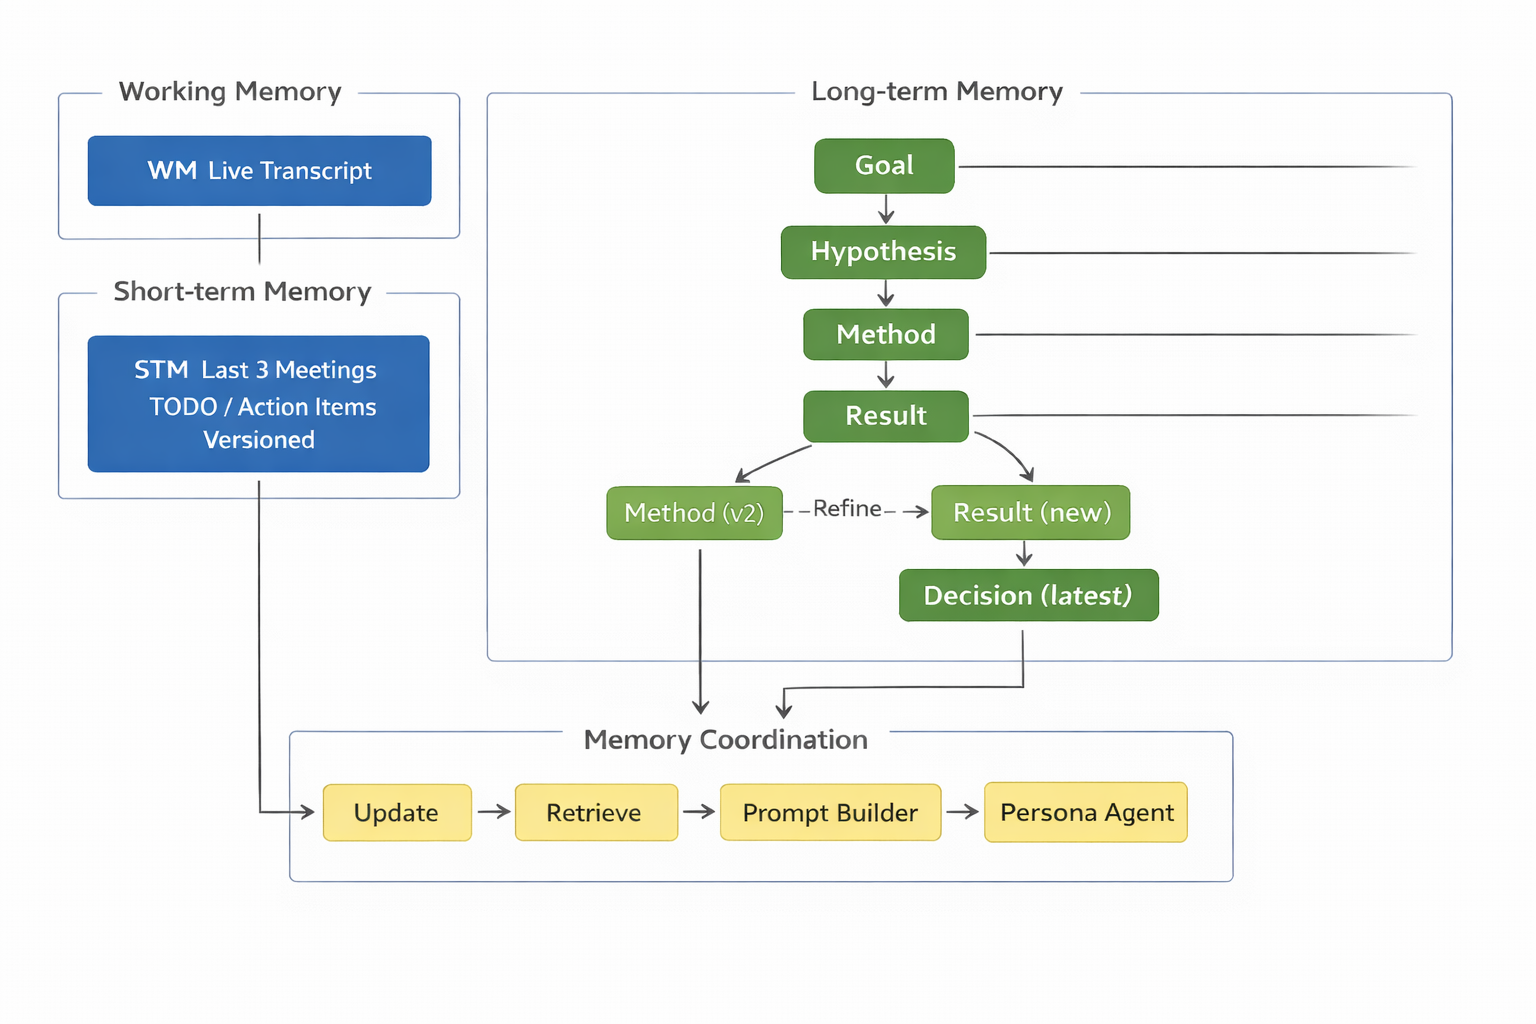
\includegraphics[width=\linewidth]{figures/memory_architecture.png}
  \caption{多層次記憶協調架構：Working/Short-term/Long-term Memory 與 Update-Retrieve 之協調流程。}
  \label{fig:memory-architecture}
\end{figure}


\subsection*{(二) 基於表徵干預之指導人設一致性監控機制（Persona Consistency Monitoring via Representation Steering）}
本研究採用 persona 表徵方向來量測「教授式導師」的人設一致性，並以推理時干預抑制 drift \citep{a2507_21509v3_personavectors}。核心作法如下：
\paragraph{(a) 自動化人設向量提取（Automated Persona Vector Extraction）}
為了獲得高保真度的 $v_{\text{professor}}$，本研究採用 Chen et al. \citep{a2507_21509v3_personavectors} 提出之自動化對比提取流程：
\begin{enumerate}
    \item \textbf{對比數據生成}：本研究自實際會議對話資料中，歸納並定義『教授式導師』之關鍵特徵描述（如學術嚴謹性、蘇格拉底式引導問答）；隨後利用大型語言模型生成 $N$ 組成對指令數據，藉由構建正、負向系統提示詞的對比，在語義空間中精準捕捉該人格特質的方向（Positive/Negative System Prompts）。
    \item \textbf{激活值採樣}：將學術問題集 $\mathcal{X}$ 輸入模型，提取模型在殘差流（Residual Stream）中的激活狀態。
    \item \textbf{向量計算}：採用均值差異法（Difference-in-Means）計算人設向量。公式如下：
    \begin{equation}
        v_{\text{professor}} = \frac{1}{|\mathcal{D}|} \sum_{x \in \mathcal{D}} \left( \mu(x)_{\text{pos}} - \mu(x)_{\text{neg}} \right)
    \end{equation}
    其中 $\mu(x)$ 代表模型生成回答時所有 token 的殘差流的平均激活值。此向量 $v_{\text{professor}}$ 即代表「學術指導人格」在激活空間中的線性方向。
\end{enumerate}
\paragraph{(b) 雙重一致性監控機制（Dual Consistency Monitoring）}
本研究建立預測性與即時性兼具的監控機制，以量化「教授式導師」的人設狀態：
\begin{itemize}
    \item \textbf{預測性監控}：在模型生成回答前，計算最後一個提示詞標記（Last Prompt Token）之激活值 $h_{\text{last}}$ 在 $v_{\text{professor}}$ 上的投影。研究證實此指標可提前預測後續生成是否偏離人設，作為預先攔截之依據 \citep{a2507_21509v3_personavectors}。
    \item \textbf{即時一致性分數}：在解碼過程中，計算每一步驟激活投影之滑動平均 $S = \text{EMA}(\langle h_l, v_{\text{professor}} \rangle)$。當 $S < \tau$ 時，視為人設偏移風險上升（如出現順從性回應傾向）。
\end{itemize}
\paragraph{(c) 推理時殘差流干預（Inference-time Steering）}
針對偵測到的人設偏移，本研究不採用重訓練模式，而是在推理時於特定層次介入殘差流，其核心更新式如下：
\begin{equation}
    h_l \leftarrow h_l + \alpha \cdot v_{\text{professor}}
\end{equation}
其中 $h_l$ 為第 $l$ 層原始激活值，$v_{\text{professor}}$ 為引導向量，$\alpha$ 為自適應干預強度係數 \citep{turner-etal-2023-activation-addition}。

\paragraph{(d) 層次選擇與自適應調整策略（Layer Selection and Adaptive Steering）}
為優化干預效率並平衡生成品質，本研究採取以下策略：
\begin{enumerate}
    \item \textbf{因果干預掃描（Causal Steering Sweep）}：透過逐層干預測試，選擇特徵表達最強且語言流暢度（Perplexity）損失最小的層次（預計為第 16--20 層）作為最終部署層 \citep{a2507_21509v3_personavectors}。
    \item \textbf{動態調整強度}：系統依據即時分數 $S$ 與閾值 $\tau$ 進行反饋調節。若 $S < \tau$，則線性調升 $\alpha$ 以強化人設立場；若一致性回歸正常，則逐步回退 $\alpha$ 以確保回覆的自然度與流暢度 \citep{wehner-etal-2025-representation-engineering}。
\end{enumerate}

\subsection*{(三) 實驗設計：自動化壓力測試與真人盲測}
\subsubsection*{1. 自動化壓力測試（Stress Tests）}
為系統化測量「邏輯一致性」與「人設漂移」，本研究設計兩類測試：

\paragraph{(a) 邏輯矛盾挑戰（Logical Contradiction Challenge）}
建立一組跨會議情境腳本：前期會議確立研究目標與方法，後期會議刻意插入矛盾訊息或錯誤前提（例如學生聲稱已完成實驗、或要求推翻先前決策但無理由）。評估指標包含：
\begin{itemize}
    \item \textbf{矛盾率（Contradiction Rate）}：以腳本標註之不可違反約束（constraints）為準，系統回覆若違反任一約束即計為矛盾，由自動衝突偵測器判定並輔以人工抽樣驗證（抽樣比例 $\ge 20\%$）。目標門檻：+Memory 相對 Baseline 矛盾率至少下降 30\%（相對下降），且絕對值 $\le 15\%$。
    \item \textbf{依賴鏈引用完整性（Dependency Chain Coverage）}：在需要引用前提的題型中，系統回覆需至少引用「前提節點」（Premise node）與「上次決策理由」兩類關鍵資訊。以自動抽取器偵測回覆中是否包含對應節點之關鍵語句或 ID，目標 coverage $\ge 80\%$。
    \item \textbf{TODO 保留率（TODO Retention Rate）}：以 TODO 之唯一識別碼（如 T01, T02）為管理單位，分母為測試起始時之有效 TODO 總數，分子為測試結束時仍正確保留之 TODO 數。允許文字改寫但 ID 不可消失或被覆寫成相反狀態。目標門檻：+Memory 條件 $\ge 90\%$，高優先 TODO 子集 $\ge 95\%$。
\end{itemize}
並以「無圖式記憶」或「僅文本記憶」作為對照，評估 Dependency Graph 的增益 \citep{a2402_17753v1_locomomemoryeval,a2505_16067v2_memorymanagementimpacts,a2602_05665v1_graphagentmemory}。

\paragraph{(b) 向量漂移量化（Persona Drift Quantification）}
以一致性分數 $S$ 的時間序列衡量 drift：比較 (i) 無干預、(ii) 固定 $\alpha$、(iii) 自適應 $\alpha$ 三種設定，並記錄：
\begin{itemize}
  \item 分數跌破閾值的頻率與持續時間；
  \item 回覆中「迎合/逢迎」觸發情境下的恢復速度（回到 $S \ge \tau$ 所需步數/回合）。
\end{itemize}
此測試用以驗證 Persona Vector Monitoring + Steering 是否能穩定抑制漂移 \citep{a2507_21509v3_personavectors,turner-etal-2023-activation-addition}。

\subsubsection*{2. 真人盲測（User Study）}
\paragraph{(a) 受試者與流程}
招募研究生（或具專題經驗之學生）進行盲測，採 within-subject 設計：每位受試者在相同任務下分別與不同系統條件互動（隨機化順序），條件包含：
\begin{enumerate}
  \item Baseline：無長期圖式記憶、無人設監控；
  \item +Memory：加入多層次記憶與 Dependency Graph；
  \item +Memory+Persona：再加入 Persona Vector 監控與自適應 steering。
\end{enumerate}

\paragraph{(b) 量表與評估面向}
以 MCA-21 量表評估「指導品質」與「互動價值」，並搭配教學能力評測架構中的各面向（如回饋可行性、引導策略、錯誤診斷與一致性）進行評分 \citep{hyun2022mca21,maurya-etal-2025-unifying}。同時參考教育對話任務評測脈絡，納入回覆的教學價值及跨回合一致性 \citep{tack-etal-2023-bea}。若資源允許，亦可將 TutorBench/TeachBench 的任務設計精神用於補充自動化指標與真人觀感的對齊 \citep{a2510_02663v1_tutorbench,a2601_21375v1_teachbench}。

\paragraph{(c) 主要假設（Hypotheses）}
\begin{itemize}
  \item H1：+Memory 條件在邏輯矛盾率、TODO 保留率上顯著優於 Baseline。
  \item H2：+Memory+Persona 條件在 persona 一致性分數與 MCA-21 指導品質上顯著優於 +Memory。
\end{itemize}

\subsection*{(四) 研究時程與里程碑（Milestones）}
\begin{enumerate}
  \item \textbf{第 1--2 月}：建立對話事件抽取、Short-term schema、Dependency Graph 資料結構與更新規則 \citep{a2602_05665v1_graphagentmemory}。
  \item \textbf{第 3--4 月}：完成檢索與一致性檢核（retrieve/check）與生成流水線整合，建立壓力測試腳本與自動化評測 \citep{a2402_17753v1_locomomemoryeval}。
  \item \textbf{第 5--6 月}：完成人設向量監控、層選擇與自適應 steering；進行 persona drift 量化測試 \citep{a2507_21509v3_personavectors}。
  \item \textbf{第 7--8 月}：真人盲測（招募、實驗執行、統計分析），完成計畫成果撰寫 \citep{hyun2022mca21,maurya-etal-2025-unifying}。
\end{enumerate}